
\loadgeometry{include}
\addtocounter{page}{-1}
\thispagestyle{empty}
\begin{center}
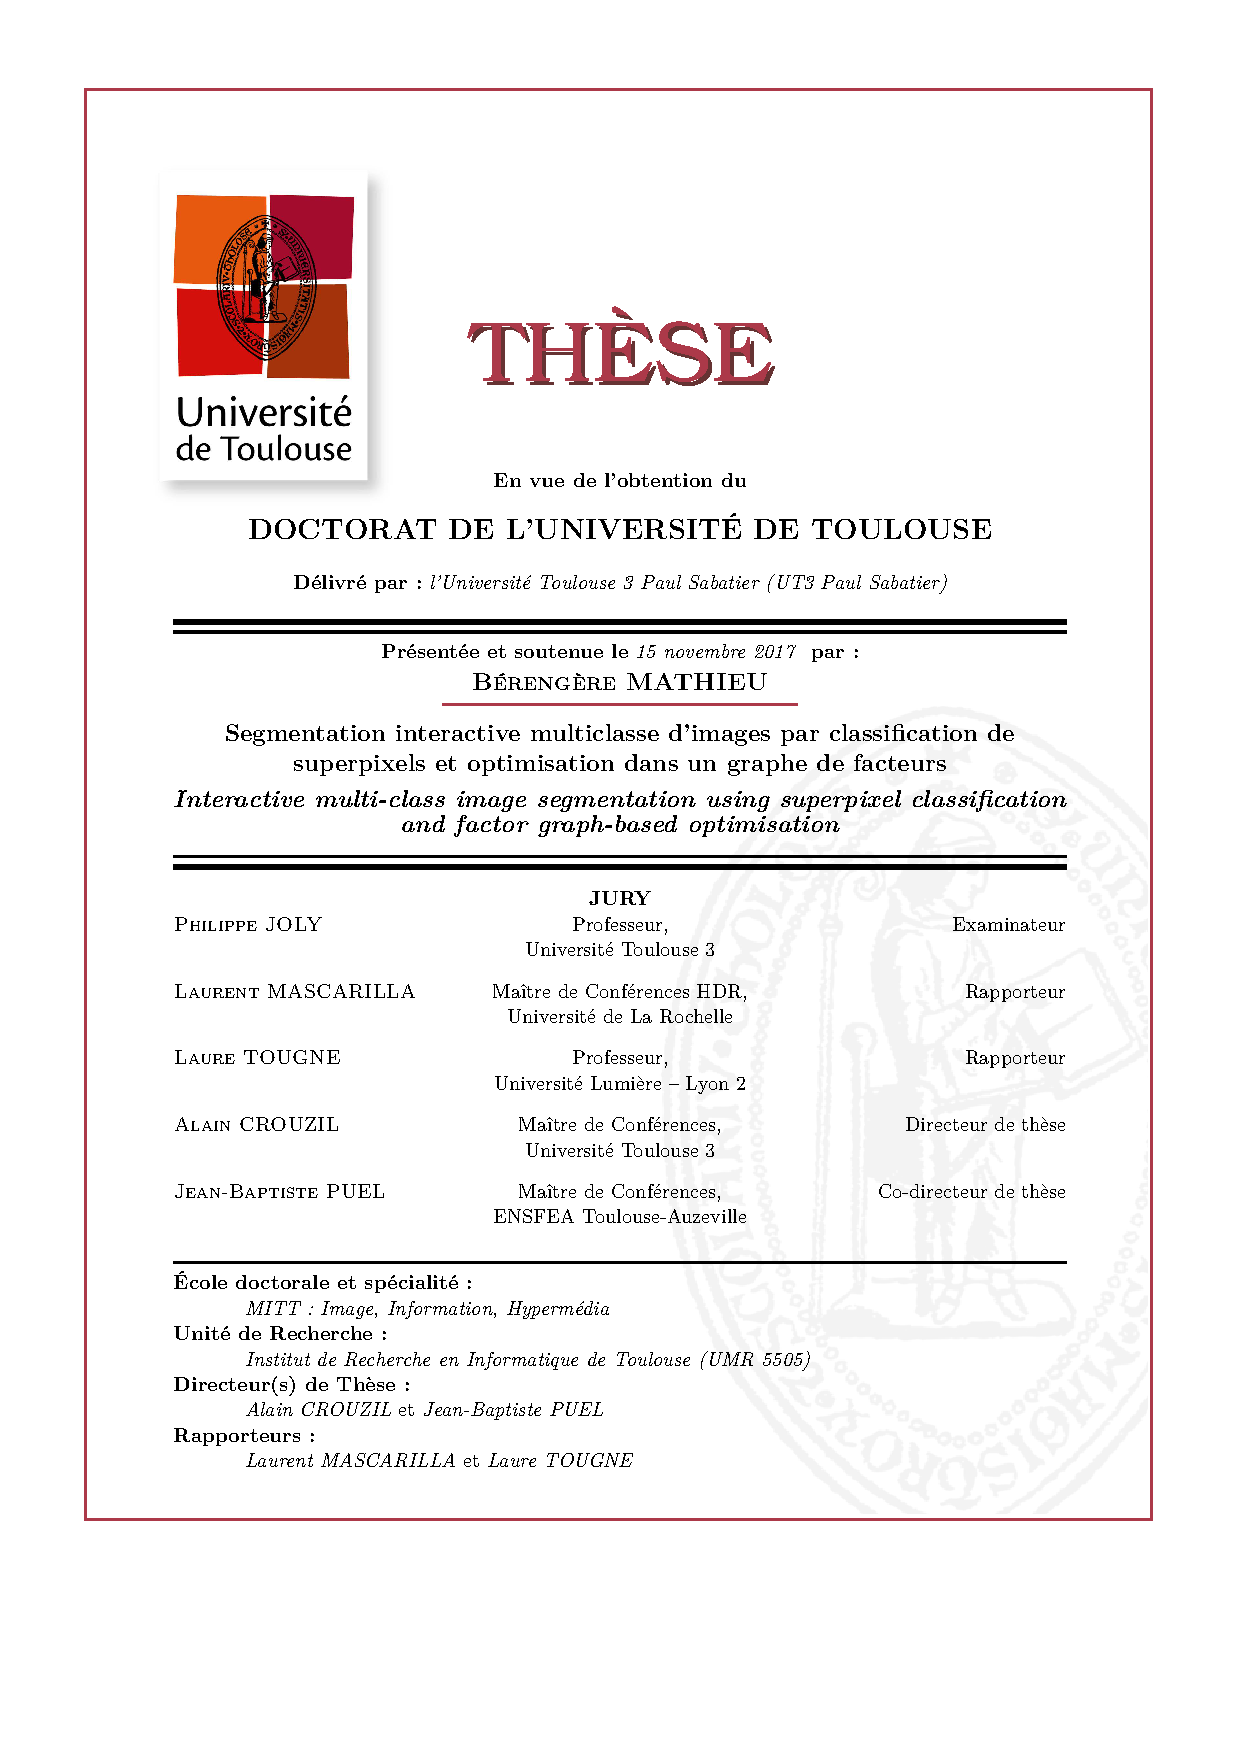
\includegraphics[width=\textwidth]{miscpages/cover-page.pdf}
\end{center}
\newpage\thispagestyle{empty}\addtocounter{page}{-1}
\loadgeometry{normalinverse}
% \addtocounter{page}{-1}
\ifthenelse {\equal{\ISDEF}{0}}
{} {

~\newpage\thispagestyle{empty}\addtocounter{page}{-1}
%%  une page de citation (pas indispensable)
 \vspace{\stretch{1}}
\vspace{0.5\linewidth}
  Avatar hocha la tête.
  \begin{itemize}
	\item[-] Ainsi, dit-il, vous avez travaillé treize longues années à rendre un idiot immortel ?   
	\item[-] La Science, dirent-ils, est au-dessus des jugements humains.
	\item[-] En ce cas devrait-elle être aux ordres de qui la nourrit ? dit Avatar. Posez ça sur la table et aller me chercher la quadrature du cercle. Comme ça, ajouta-t-il, une fois les savants partis tout perplexes, pendant ce temps-là ils ne feront pas de mal.
	\item[ ] Et qu'est-ce que je vais en faire, dit-il en tournant dans sa main le flacon. Car enfin, qui voudra sauver sa vie ne la perdra-t-il pas ?
	\item[ ] Et d'un bras ferme il expédia à travers la fenêtre la sombre fiole, qui avec un joyeux plouc tomba au fond des douves.
  \end{itemize} 
\begin{flushright}
  Christiane Rochefort,  \emph{Archaos ou le jardin étincelant}\\
 % par bob
\end{flushright}
\vspace{\stretch{2}}

%% Encore une page blanche pour que les remerciements arrivent
%%  sur une page impaire

\newpage\thispagestyle{empty}\addtocounter{page}{-1}
~\newpage\thispagestyle{empty}\addtocounter{page}{-1}

\section*{Remerciements}

Ce mémoire contient la synthèse de trois années de travail scientifique. Il est dédié à tout celles et ceux qui m'ont accompagnée, épaulée, secouée, précipitée, rattrapée. Tous, je les remercie du fond du cœur.

\begin{itemize}[label=\ ]
\item Adrian, pour l'avoir entraîné au moins deux fois dans les boutiques Lush 
\item Agnès, pour ouvrir une fenêtre sur un peu de douceur, quelque part dans le Périgord
\item Anahid, sa force de caractère et son calme,  
\item Alain, dont les qualités humaines ont nourris ma motivation alors que tout autre denrée venait à manquer
\item Amélie, dont j'espère que les œuvres rencontreront le succès qu'elles méritent 
\item Arturo, mon ami de l'autre côté de la terre
\item Aurélie, avec tous mes vœux de bonheur 
\item Anne, pour s'être taillé à la serpe un chemin dans les épines sans jamais éteindre la braise 
\item Bérénice, artiste, boulangère, informaticienne 
\item Camille, pour son infinie compassion 
\item Carole, pour la liberté qu'elle nous a accordé lorsque nous accompagnions vers la réussite
\item Christian, puisqu'il s'en ait passé du temps depuis qu'assise sur ses genoux je tapais "papa" sur le clavier
\item Christine, marraine et femme reine
\item Christine, m'ARM 
\item Christophe, pour avoir accueillit chez lui nos adieux à Artuto
\item Christophe, pour une traversée du Rhin dans la nuit glacée de décembre 
\item Clément, compagnon d'humour noir
\item Corentin, esprit libre dont j'ai hâte de découvrir les fruits,
\item Damien, pour avoir été garçon et mathématicien, dans notre groupe de filles informaticiennes
\item Damien, avec mes meilleurs vœux pour ses projets de médiation scientifique 
\item Damien, pour m'avoir apprivoisé en conférence
\item Denis, pour ses idées de repas d'équipe 
\item Églantine, dont j'aime tant l'esprit scientifique et la générosité
\item Émeline, dont la fougue secoue le monde pour en faire tomber les fruits
\item Érick, pour sa fraîcheur de jeune chercheur
\item Faustine, dont la rigueur et le calme m'impressionneront toujours
\item Isabelle, pour la place qu'elle m'a laissé occupée au sein du labex 
\item Jean-Baptiste, spécialiste en tout
\item Josiane, et ses festins de Babette
\item Florent, et longue vie aux hamsters
\item Florent, qui je l'espère conservera toujours son enthousiasme et sa curiosité 
\item Jean-Pierre, pour s'être intéressé à la question humain et y avoir répondu par Makina 
\item Jessica, qui a enlevé les pierres qui m’empêchaient de jaillir 
\item Joseph, qui rend le monde un peu meilleur 
\item Julie, la Culottée que j'aurais rencontrée 
\item Laura, en lui souhaitant une longue carrière dans l'enseignement 
\item Laure, pour sa bienveillance et son enthousiasme vis-à-vis de mes travaux 
\item Laurent, pour son patient travail de relecture 
\item Lisa, qui découvrira sa force lorsque le printemps réveillera la sève
\item Lise, pour son altruisme  
\item Ludwig, qui sait que aimer c'est être possédé
\item Martin, pour avoir rendu possible les camps d'étés de CIMI
\item Marine, en lui souhaitant qu'en haut du tableau, le bambou ne soit pas seul
\item Martine, qui m'a transmis l'écriture comme les premiers hommes transmettaient le feu à leurs enfants 
\item Mélisa, la grande cousine que j'admirerai toujours
\item Mohamat,qui fera un chercheur brillant 
\item Michel, qui m'a appris à laisser de la place pour l'Himalaya 
\item Ophélie, dont les cheveux roses sont comme un puits dans le désert 
\item Nadia, là bas près de l'océan 
\item Philippe, pour sa douceur et sa gentillesse
\item Romain, qui a su me redonner le goût de la photographie
\item Roman, pour m'avoir fait découvrir l'art numérique
\item Rosa, en lui souhaitant tout le succès qu'elle mérite
\item Sandra, avec tous mes vœux de réussite
\item Sandrine, pour m'avoir laissé jouer avec ses drones
\item Shaé, chat infernal de son état  
\item Serge, l'oncle qui danse le jerk 
\item Téodora, funambule entre les langues étrangères
\item Tom, à la mémoire du poulpe fou qui tweet de la politique
\item Yannick, pour ses conseils 
\item Yeu, à qui je dois ma première publication dans une revue
\item Yohan, que j'aime comme les arbres aiment la source qui baigne leurs racines
\item Zélie, qui sait tout comprendre. 
\end{itemize}

\newpage\thispagestyle{empty}\addtocounter{page}{-1}

\newpage\thispagestyle{empty}
~\newpage\thispagestyle{empty}


}


\loadgeometry{normal}


